\section{Durchführung}
\label{sec:Durchführung}

\subsection{Teil 1}
Insgesamt besteht das Experiment aus 2 Teilen. Im Ersten geht es um die 
Apparatur wie in \autoref{fig:teil1} dargestellt. Gemessen wird in einem 
Bereich von 30 mbar bis 1 bar. Für die Bestimmung der Dampfdruckkurve von 
Wasser wird als erstes die Wasserstrahlpumpe evakuiert. Bedingung dafür sind 
geschlossene Belüftungsventile, währenddessen sind Absperrhahn und Drosselventil 
geöffnet. Der Druck verringert sich, der Enddruck wird erreicht. Nun werden 
Wasserstrahlpumpe, Absperrhahn und Drosselventil wieder verschlossen. Die 
Woulffsche Flasche hat hierbei nur einen Präventationszweck: Sie sorgt dafür, 
dass beim Abstellen des Wassereinlasses kein Wasser in die evakuierte Apparatur 
eindringt. Im Anschluss werden Kaltwasserzufuhr und Heizhaube eingeschaltet, 
sodass das Wasser anfängt zu sieden. Es werden dazu zahlreiche Temperaturen 
in Abhängigkeit des Drucks dokumentiert.
\begin{figure}[h!]
    \centering
        \centering
        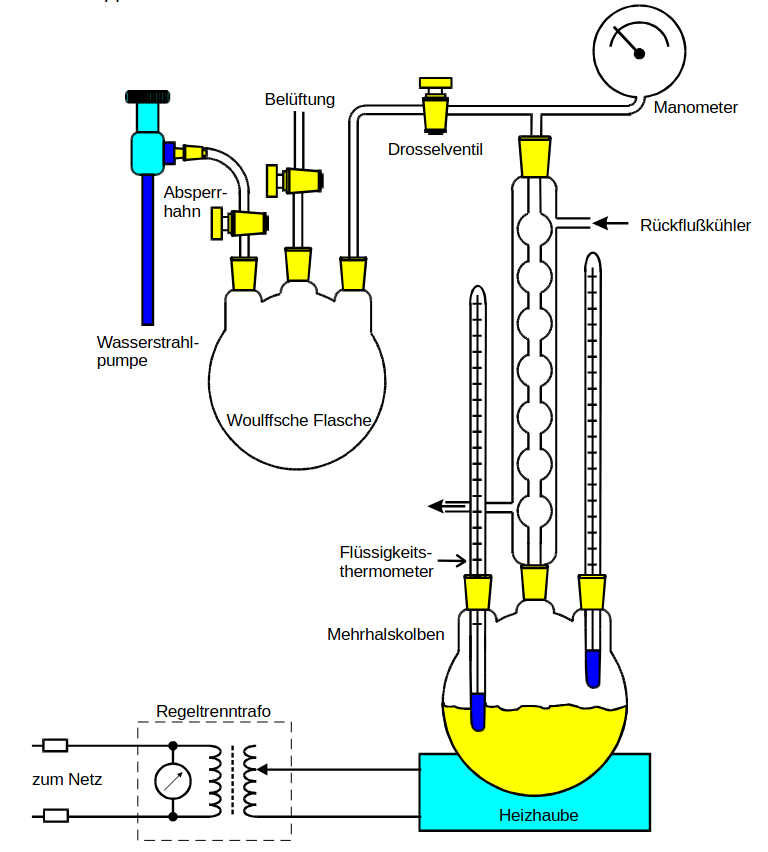
\includegraphics[width=\textwidth]{Bilder/teil1.png}
        \caption{Messapparatur für einen Druck $p \leq$ 1 bar \cite{teil1}}
    \hfill
    \label{fig:teil1}
\end{figure}
\\
\\
\\
\\
\\
\\
\\
\\
\\
\\
\\
\\
\subsection{Teil 2}
Im 2. Teil soll nun die Dampfdruckkurve mittels der in \autoref{fig:teil2} zu 
sehenden Apparatur bestimmt werden. Diese beinhaltet im Hohlraum des durchbohrten 
Stahlbolzens das Wasser. Weiterhin ist das Innere verknüpft mit einem U-Rohr, 
welches wiederum mit dem Drucksensor verbunden ist. Um das Rohr herum befindet 
sich die Heizwicklung, welche das Rohr erhitzen soll. Sobald ein Druck von 1 bar 
erreicht ist beginnt die Messung. In einem Abstand von 1 bar wird die Temperatur 
gemessen, bis 15 bar erreicht sind.
\begin{figure}[h!]
    \centering
        \centering
        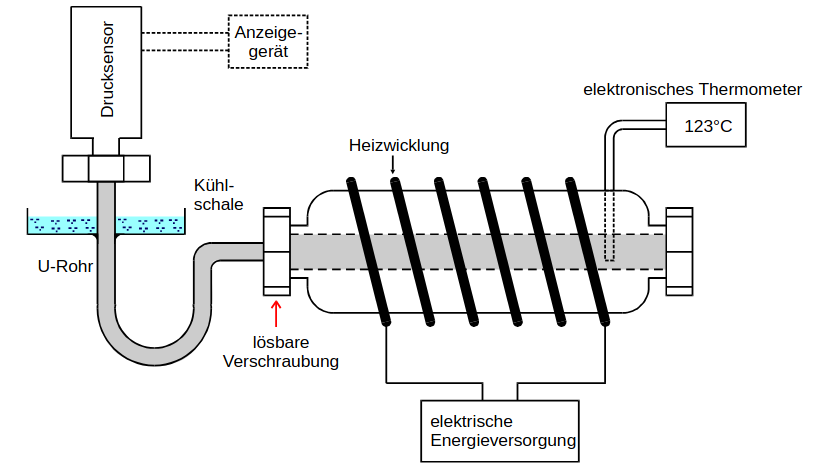
\includegraphics[width=\textwidth]{Bilder/teil2.png}
        \caption{Messapparatur für einen Druck $p$ < 1 bar \cite{teil2}}
    \hfill
    \label{fig:teil2}
\end{figure}